\chapter{Analisi}
Il presente capitolo fornisce un'analisi introduttiva sul sistema legacy, descrivendone le funzionalità principali, l'architettura e le tecnologie impiegate. Verranno evidenziati i limiti strutturali e operativi che hanno portato l'azienda a intraprendere un processo di reingegnerizzazione, con l'obiettivo di sviluppare un sistema più moderno, scalabile e manutenibile.

Un aspetto cruciale di questa analisi riguarda la strategia di transizione dal sistema legacy al nuovo pannello di configurazione. Inizialmente era stata prevista una coesistenza graduale tra i due sistemi, ma la direzione aziendale ha successivamente deciso di adottare un approccio differente. Il nuovo sistema verrà sviluppato fino a includere tutte le macrofunzionalità fondamentali, che gli garantiranno una quasi completa operatività. Inoltre, sarà introdotta una nuova funzionalità che, oltre a rappresentare un'evoluzione rispetto al legacy, contribuirà a differenziare il nuovo sistema e a valorizzarne le potenzialità.
%
Solo una volta completato, il nuovo pannello sostituirà integralmente il legacy con una transizione netta, eliminando quindi la necessità di retrocompatibilità e riducendo la complessità della fase transitoria.

Proseguendo, il capitolo illustrerà gli obiettivi e i requisiti principali che hanno guidato la progettazione del nuovo sistema, preparando la discussione del capitolo successivo, in cui verranno descritte nel dettaglio le scelte architetturali adottate per superare le limitazioni del sistema legacy e rispondere alle nuove esigenze aziendali e di mercato.

Infine, la parte finale del capitolo sarà dedicata all'analisi del dominio applicativo, con l'obiettivo di identificare i concetti e le entità fondamentali del sistema legacy che verranno utilizzati per la progettazione del nuovo sistema. Questa analisi è essenziale per definire una base strutturata su cui modellare le funzionalità del nuovo pannello di configurazione, garantendo una transizione coerente e ben organizzata dalle logiche del sistema precedente a quelle della nuova implementazione.

\section{Introduzione al sistema esistente}
Il sistema legacy qui esaminato rappresenta un pannello Web utilizzato dall'azienda \textit{FlashStart Group srl}\footnote{\url{https://flashstart.com}} per la gestione e la configurazione del suo filtro DNS. L’analisi di questo sistema, effettuata nell’ambito di un tirocinio in preparazione della presente tesi, si basa sulle osservazioni dirette fatte durante lo sviluppo del nuovo sistema, dato che la documentazione del legacy risulta pressoché assente.

\subsubsection{Terminologia e definizioni}
Da qui in avanti verranno utilizzate alcune terminologie specifiche che descrivono concetti e funzionalità del sistema legacy. Pertanto, prima di proseguire con la sua analisi, è opportuno fornire una breve spiegazione di questi termini, utilizzati dall'azienda per rappresentare concetti chiave del dominio applicativo.

\begin{itemize}
  \item \textbf{Rete}: identifica un indirizzo IP registrato nel sistema e associato alla sede di un cliente, come ad esempio una scuola. Le reti possono essere statiche (IP pubblico fisso) o dinamiche (IP pubblico variabile).

  \item \textbf{Endpoint}: rappresenta un dispositivo fisico specifico registrato nel sistema, come un computer o uno smartphone. A differenza della rete, un endpoint è associato direttamente a un dispositivo, piuttosto che a un indirizzo IP generico.

  \item \textbf{Dealer}: un rivenditore che vende licenze del filtro DNS ai clienti finali, i quali devono, in autonomia, configurare le proprie policy di sicurezza tramite il pannello Web.

  \item \textbf{Managed Service Provider (MSP)}: è un particolare tipo di Dealer che, oltre a vendere licenze, si occupa anche della configurazione e della gestione delle policy di sicurezza per i propri clienti. A differenza dei precedenti fornitori di servizi, gli MSP impediscono ai clienti finali di accedere al pannello, occupandosi interamente della gestione.

  \item \textbf{Whitelabel}: una funzionalità che consente ai fornitori di servizi, come gli MSP, di personalizzare il pannello Web con il proprio logo, colori e branding, nascondendo ogni riferimento al produttore originale del sistema.

  \item \textbf{ClientShield}: Un'applicazione per computer e dispositivi mobili sviluppata dall'azienda, che consente di registrare un endpoint nel sistema e sfruttare il filtro DNS anche al di fuori della rete usuale.
\end{itemize}

\subsection{Panoramica sulle funzionalità}
Il pannello Web legacy rappresenta lo strumento principale per la gestione e configurazione del filtro DNS offerto dall'azienda. Nonostante le limitazioni architetturali e tecnologiche, il sistema fornisce un insieme di funzionalità che consentono agli utenti di configurare, monitorare e amministrare le policy di filtraggio DNS. Di seguito viene fornita una panoramica delle principali funzionalità offerte dal suddetto pannello.

\subsubsection{Gestione delle policy di protezione}
Il pannello consente di creare e configurare diversi profili di protezione, ciascuno dei quali può includere una combinazione personalizzata di filtri per:
\begin{itemize}
  \item Bloccare minacce informatiche come malware e phishing;
  \item Limitare l'accesso a contenuti specifici, come siti per adulti o contenuti inappropriati;
  \item Bloccare l'accesso ad applicazioni o servizi specifici, divisi per categoria di appartenenza;
  \item Bloccare l'accesso a pagine Web e servizi provenienti da determinate aree geografiche.
\end{itemize}
Per aumentare il grado di flessibilità del filtro, gli utenti possono creare delle liste di accesso personalizzate, tra cui:
\begin{itemize}
  \item \textbf{Allow list}: per consentire l'accesso a domini specifici;
  \item \textbf{Block list}: per bloccare domini o indirizzi IP specifici.
\end{itemize}
Queste liste possiedono una priorità più elevata rispetto alle funzioni di protezione citate in precedenza. Per questo motivo, esse consentono di specificare delle eccezioni rispetto alle normali policy di sicurezza. Ad esempio, è possibile concedere l'accesso ad un contenuto di norma non consentito, oppure bloccare un dominio che risulta legittimo.

\subsubsection{Gestione delle reti di protezione}
Un'altra funzionalità fondamentale del pannello è la possibilità di specificare quali reti devono essere sottoposte al filtraggio, garantendo un controllo preciso e mirato sulle attività DNS. Questo permette di configurare reti aziendali o domestiche in modo che tutte le richieste DNS generate da tali indirizzi IP passino attraverso le policy di protezione impostate. La configurazione delle reti di protezione può essere adattata a diverse esigenze, supportando due principali modalità:
\begin{itemize}
  \item \textbf{IP pubblico statico}: questa configurazione è utilizzata quando la rete dispone di un IP pubblico statico, ovvero un indirizzo IP assegnato in modo permanente dal proprio ISP. In questo caso, il pannello consente di associare le policy di filtraggio a una rete identificata da uno specifico IP, garantendo che tutte le richieste DNS provenienti da tale rete siano sottoposte ai controlli e ai filtri impostati;

  \item \textbf{IP pubblico dinamico}: per le reti che non dispongono di un IP pubblico statico, il sistema supporta la configurazione tramite DynamicDNS\footnote{\url{https://www.rfc-editor.org/rfc/rfc2136.html}} (DDNS). Questo approccio consente di monitorare e filtrare le richieste DNS anche quando l’indirizzo IP della rete varia nel tempo, utilizzando un sistema di aggiornamento dinamico che associa un nome di dominio all’IP corrente della rete. Questo garantisce continuità nella protezione senza la necessità di aggiornamenti manuali;
\end{itemize}

\subsubsection{Visualizzazione e analisi dei report}
Il pannello offre una sezione dedicata alla generazione e analisi dei report relativi al traffico DNS della rete, permettendo di monitorare l’efficacia delle policy di filtraggio e di ottenere informazioni dettagliate sull’attività di rete in un determinato intervallo di tempo. Questi report forniscono una visione chiara e organizzata del comportamento della rete, aiutando gli utenti a identificare potenziali minacce e a ottimizzare le configurazioni esistenti.

\paragraph{Tipologie di report disponibili}
Tramite un menù a cascata, è possibile selezionare diversi tipi di report, tra cui:
\begin{itemize}
  \item \textbf{Bloccati per categoria}: mostrano le richieste DNS bloccate verso siti indesiderati, raggruppandole per categoria o macro-categoria;
  \item \textbf{Consentiti per paese o categoria}: forniscono il numero di richieste consentite, organizzate per paese o per categoria di contenuti;
  \item \textbf{Malware e minacce bloccate}: presentano un’analisi delle richieste che hanno attivato il filtro, indicando malware o altre minacce bloccate;
  \item \textbf{Traffico per fasce orarie o giorni}: permettono di analizzare le richieste DNS effettuate in specifiche fasce orarie o giorni della settimana;
  \item \textbf{Report geografici}: forniscono una mappa del mondo che evidenzia il traffico DNS suddiviso per paesi e continenti.
\end{itemize}

Dopo aver configurato i parametri di analisi, gli utenti possono generare i report secondo diverse modalità. Essi possono essere esportati in formato PDF, oppure inviati direttamente via e-mail a destinatari predefiniti. Inoltre, il pannello offre una funzione di pianificazione che consente di programmare l'invio automatico dei report a intervalli regolari, ad esempio su base settimanale, rendendo più efficiente il monitoraggio continuo.

\subsubsection{Gestione dei dispositivi protetti (Endpoint)}
Il pannello include anche una funzionalità per gestire i dispositivi su cui è installato il ClientShield. In particolare, questa configurazione permette di tracciare con precisione quale dispositivo ha originato una determinata richiesta DNS, fornendo un maggiore controllo e un livello di dettaglio maggiore sulle attività della rete.

\subsubsection{Funzionalità aggiuntive}
Oltre alle funzionalità principali già descritte, il pannello Web offre una serie di strumenti utili per migliorare la gestione e il controllo delle configurazioni. Tra queste, vi è la possibilità di personalizzare la pagina di blocco che viene visualizzata dagli utenti ogni volta che tentano di accedere a un dominio non consentito.
%
Il pannello consente anche di verificare facilmente a quale categoria appartiene un determinato sito Web, aiutando gli utenti a valutare come configurare al meglio le politiche di filtraggio.
%
Un’altra funzionalità interessante è la visualizzazione del traffico DNS in tempo reale, che fornisce un monitoraggio immediato dell’attività di rete. Inoltre, il sistema supporta l'importazione di domini in formato batch, permettendo di aggiungere rapidamente liste di siti Web consentiti o bloccati attraverso file di testo.

Per concludere la panoramica sulle funzionalità, il pannello possiede un'importante integrazione con la tecnologia Active Directory di Microsoft, che consente di ottenere informazioni dettagliate non solo sul dispositivo che ha originato una determinata richiesta DNS, ma anche sull’utente utilizzato per accedere a tale macchina.

\subsection{Architettura e tecnologie utilizzate}
Il pannello Web in esame, fino ad ora descritto solo dal punto di vista delle funzionalità, presenta un'architettura monolitica, tipica dei vecchi sistemi Web-based. Nonostante sia possibile identificare due macro-sezioni, denominate \textit{Customer area} e \textit{Pannello cloud}, non vi è una reale modularizzazione del frontend e del backend. Tutto il codice risulta scritto in modo procedurale, senza l’adozione di un paradigma orientato agli oggetti, e con una scarsa separazione delle responsabilità.

\subsubsection{Tecnologie utilizzate}
Il backend è interamente sviluppato in PHP, utilizzando un approccio ``plain'', ossia privo di framework moderni come Laravel\footnote{\url{https://laravel.com}}. Per il frontend sono stati utilizzati HTML, CSS e una versione obsoleta di jQuery\footnote{\url{https://jquery.com}} (\texttt{1.x}), che limita le possibilità di modernizzazione dell'interfaccia. In alcuni casi, il codice PHP si occupa anche di generare dinamicamente script JavaScript, i quali eseguono ulteriori chiamate a codice PHP lato server.

\subsubsection{Integrazione con API esterne}
L'azienda ha sviluppato un set di API pubbliche che consentono di gestire il filtro DNS senza dover necessariamente utilizzare il pannello Web in questione. Queste API offrono agli utenti la possibilità di integrare il filtro DNS in applicazioni personalizzate o di sviluppare un proprio client per la gestione delle configurazioni.

Nel tempo, alcune operazioni che il sistema legacy eseguiva direttamente sono state trasferite alle suddette API, le quali centralizzano la business logic e gestiscono l'interazione con il database. Il pannello Web, in questi casi, funge da semplice interfaccia per chiamare le API. Tuttavia, molte operazioni continuano a risiedere direttamente sul sistema, implementando la logica applicativa e accedendo alla base dati.

\subsubsection{Gestione del database}
Il sistema legacy utilizza due database distinti per gestire le sue funzionalità e garantire la persistenza delle configurazioni. Entrambi adottano un motore di database \emph{relazionale}, che organizza i dati in tabelle collegate tra loro tramite un sistema di chiavi. La differenza principale risiede nella tecnologia sottostante: una base dati utilizza MySQL\footnote{\url{https://www.mysql.com}}, mentre l’altra è basata su PostgreSQL\footnote{\url{https://www.postgresql.org}}. Ciascuna di esse è destinata a scopi specifici e presenta caratteristiche diverse in termini di configurazione e prestazioni.

Il database MySQL è dedicato esclusivamente alla gestione delle licenze e dei dati anagrafici dei clienti. Esso viene ospitato su un server interno all’azienda e non è replicato in altre regioni. Questa configurazione rappresenta un collo di bottiglia significativo per gli utenti distanti dalla sede aziendale, poiché tutte le richieste relative ai dati dei clienti o delle licenze (usate soprattutto nella fase di accesso al pannello) devono necessariamente essere inviate al server centrale per essere elaborate, causando latenze elevate.

Il database PostgreSQL, invece, è utilizzato per tutti gli altri dati, inclusi i report, le regole di protezione e le liste dei domini da bloccare. Questo database è configurato in replica globale, garantendo così prestazioni più elevate e tempi di risposta migliori per i clienti situati in diverse aree geografiche. Grazie a questa configurazione, i dati necessari al funzionamento del filtro DNS possono essere accessibili rapidamente da qualunque parte del mondo.

Un aspetto di fondamentale importanza per l'azienda è rappresentato dal contenuto del suddetto database, che costituisce un valore strategico significativo. Al suo interno, infatti, è presente una lista dei domini associati alla relativa categoria di appartenenza. Questa categorizzazione è utilizzata direttamente dal filtro DNS per bloccare l'accesso a determinati siti in base alle regole configurate dagli utenti. L'operazione di categorizzazione viene gestita internamente all'azienda e si basa su un approccio di intelligenza artificiale. Tale sistema analizza i testi delle pagine Web e determina automaticamente la categoria di appartenenza di ciascun dominio, migliorando l'efficacia del filtro DNS e arricchendo continuamente il patrimonio informativo del database.

\subsection{Limitazioni riscontrate}
Il sistema legacy presenta numerose limitazioni che hanno reso necessaria una completa reingegnerizzazione. Queste riguardano sia l’assenza di funzionalità fondamentali, come il supporto alla multiutenza, sia problematiche strutturali e di usabilità che compromettono la flessibilità e l’efficienza operativa dello stesso.

\subsubsection{Mancanza del supporto alla multiutenza}
Una delle principali limitazioni del sistema legacy, e tra quelle più sentite dai clienti dell'azienda, è l’assenza di un supporto per la multiutenza. Attualmente, infatti, il sistema permette a ciascun cliente di disporre di un unico account per accedere al pannello di configurazione, che possiede i privilegi di amministratore.

Questa mancanza rappresenta un ostacolo significativo, soprattutto per i dealer o gli MSP che integrano il filtro DNS in altri prodotti o lo rivendono ad aziende terze. Questi ultimi si trovano spesso a dover gestire configurazioni e politiche di protezione per conto dei loro clienti, ma l'assenza di un sistema multiutente impedisce di delegare determinate operazioni o di offrire accesso limitato a figure specifiche all’interno delle organizzazioni servite. Allo stesso modo, chi utilizza direttamente il pannello non può creare profili con permessi ridotti, ad esempio per utenti che necessitano soltanto di monitorare le configurazioni o consultare i report senza possibilità di modificarli.

Implementare la funzionalità in questione nel sistema attuale richiederebbe modifiche strutturali profonde, che non sono realisticamente attuabili senza un suo completo stravolgimento.

\subsubsection{Profili di protezione non condivisibili}
Un’altra significativa limitazione del sistema legacy riguarda l’impossibilità di condividere i profili di protezione tra diversi utenti. Attualmente, ogni profilo è strettamente associato a un singolo cliente, senza alcuna possibilità di essere condiviso o ereditato da altri. Questa carenza rappresenta un ostacolo rilevante, specialmente per gli MSP che gestiscono clienti con esigenze simili, come un gruppo di scuole o aziende dello stesso settore. In tali casi, sarebbe estremamente utile disporre di profili condivisi che consentano di applicare la stessa configurazione a più clienti contemporaneamente.

Inoltre, la mancanza di questa funzionalità aumenta il carico di lavoro in caso di modifiche alle regole di protezione. La situazione attuale, infatti, è tale per cui ogni variazione deve essere riportata manualmente su ciascun cliente, imponendo un processo lungo e soggetto a errori.

\subsubsection{Limiti e debolezze architetturali}
Il sistema legacy presenta numerosi limiti dovuti a scelte architetturali e tecnologiche datate, che influiscono negativamente sulla manutenibilità e sull'evoluzione del software. La mancanza di una chiara separazione tra frontend e backend complica la gestione del codice, rendendo difficoltosa l’adozione di nuove tecnologie. Oltretutto, pratiche quali l’utilizzo di PHP per generare dinamicamente codice JavaScript introducono ulteriore complessità ed opacità dei sorgenti, limitando la modularità e aumentando il rischio di commettere errori.

L’architettura monolitica rappresenta una delle principali debolezze del sistema. Qualsiasi modifica, anche minima, comporta interventi che possono avere ripercussioni su altre parti del codice, a causa dell’assenza di un design accurato e di una netta separazione delle responsabilità. Questo approccio non solo rallenta il ciclo di sviluppo, ma aumenta significativamente il rischio di regressioni e rende difficoltoso il debugging. La mancanza di modularità aggrava ulteriormente il problema: ogni nuova funzionalità o aggiornamento richiede un lavoro complesso e rischioso, che spesso si traduce in un incremento della fragilità del sistema.

\subsubsection{Problemi di usabilità}
L'interfaccia utente del sistema, sviluppata con tecnologie ormai obsolete, presenta diverse limitazioni che compromettono l’esperienza degli utenti finali. L’utilizzo di una versione datata di jQuery, unito all’assenza di un layout moderno, rende l’interfaccia poco intuitiva e difficoltosa da navigare. Questi problemi non solo riducono l’efficienza operativa degli utenti, ma influenzano negativamente anche la percezione complessiva del sistema.

Un design grafico superato e poco efficiente limita inoltre la capacità del sistema di competere con soluzioni contemporanee, riducendone l’attrattiva sia per gli utenti attuali che per potenziali nuovi clienti.

\subsubsection{Conclusione}
Le limitazioni evidenziate, che includono l’assenza di funzionalità essenziali come la multiutenza e i profili condivisibili, le debolezze architetturali e i problemi legati all’usabilità e all’interfaccia utente, mettono in luce la rigidità e l'obsolescenza del sistema legacy. Tali carenze ostacolano non solo l'efficienza operativa e la scalabilità del sistema, ma anche la capacità dell'azienda di rispondere alle richieste di mercato e di competere con soluzioni moderne. Questi fattori rendono indispensabile una completa reingegnerizzazione per soddisfare le esigenze attuali e future, garantendo al contempo un sistema moderno, scalabile ed efficiente.

\section{Esigenze di transizione tra i due sistemi}
La transizione dal sistema legacy al nuovo pannello di configurazione seguirà una strategia differente rispetto a quanto inizialmente previsto. Non sarà più adottato un approccio di coesistenza graduale tra i due sistemi, bensì una transizione netta non appena il nuovo sistema sarà pronto per il rilascio. Durante la fase di sviluppo, il vecchio pannello rimarrà l’unico utilizzato dagli utenti, mentre il nuovo verrà completato fino a includere tutte le macrofunzionalità fondamentali necessarie per garantirne l’operatività, oltre a una nuova funzionalità dedicata alla gestione dei profili condivisi. Solo a quel punto avverrà il passaggio definitivo al nuovo sistema.

Poiché gli utenti si ritroveranno i propri dati direttamente nel nuovo pannello, la migrazione delle informazioni dal legacy al nuovo sistema diventa un requisito fondamentale. Questo processo avverrà internamente all’azienda e dovrà garantire che tutti i dati necessari alle funzionalità trasferite siano disponibili nel nuovo sistema prima del rilascio. Le strategie di migrazione adottate dovranno assicurare la completa integrità e coerenza delle informazioni, evitando perdite o incongruenze tra i due ambienti.

Dopo il rilascio, la fase di transizione sarà limitata esclusivamente al periodo necessario per completare il trasferimento delle funzionalità minori ancora rimaste nel legacy. Tuttavia, rispetto all'approccio iniziale, non sarà più richiesta alcuna retrocompatibilità tra i due sistemi. Infatti, le funzionalità che continueranno a essere utilizzate nel legacy fino alla loro migrazione definitiva non dovranno interagire con il nuovo sistema, evitando così complessità aggiuntive nella gestione dei dati.

Questa strategia di transizione consente di semplificare il passaggio al nuovo sistema, evitando la necessità di mantenere attivi entrambi i pannelli per un lungo periodo. Inoltre, riduce i rischi legati alla gestione della retrocompatibilità e permette di concentrare gli sforzi sullo sviluppo del nuovo sistema senza vincoli imposti dall’integrazione con il legacy.

\section{Analisi del nuovo sistema}
\subsection{Obiettivi}
Il nuovo sistema nasce con l'obiettivo di posizionarsi come una soluzione moderna e professionale, capace di soddisfare le esigenze di un mercato in espansione e di attirare anche clienti di grandi dimensioni. Per raggiungere questo scopo, è fondamentale che il pannello abbia un'interfaccia più curata e in linea con gli standard richiesti da organizzazioni complesse. Questo aspetto si inserisce in un più ampio percorso di rinnovamento della \textit{brand identity} aziendale, che include un nuovo logo, una palette di colori aggiornata e uno stile comunicativo uniforme.

Dal punto di vista tecnico, il sistema dovrà superare le limitazioni strutturali del legacy, modernizzando l'architettura per renderla più robusta e scalabile, in modo da poter gestire un numero crescente di utenti. Una delle priorità è quella di ridurre i tempi necessari per la manutenzione e l’aggiornamento, facilitando al contempo l’integrazione di nuove funzionalità.

Un obiettivo chiave della prima release del pannello è l'introduzione di funzionalità avanzate pensate per i fornitori di servizi, con particolare attenzione ai dealer e agli MSP. Tra queste, un ruolo centrale è ricoperto dai profili condivisi, noti anche come \textit{template}, che consentono di definire e applicare regole di protezione comuni a più clienti. Grazie ad i template, gli MSP potranno gestire in modo più efficiente le configurazioni, evitando di doverle replicare manualmente per ciascun cliente e permettendo la propagazione automatica delle modifiche.
%
Un'altra caratteristica fondamentale che differenzia questa prima versione da quella legacy è la presenza di una dashboard dedicata ai fornitori di servizi gestiti. Questo strumento consentirà loro di gestire in maniera completa ed efficace i clienti sotto la loro supervisione, offrendo una panoramica dettagliata sul traffico, sulle configurazioni applicate e sugli eventi di sicurezza rilevati. La dashboard sarà progettata per agevolare l’amministrazione su larga scala, semplificando operazioni come la modifica delle policy di protezione, l'assegnazione dei template e il monitoraggio centralizzato delle reti gestite.

Infine, una funzionalità fondamentale che differenzia questa prima versione da quella legacy è la gestione avanzata della multiutenza, una caratteristica assente nel sistema precedente. Nel nuovo pannello, sarà possibile associare più utenti a un singolo cliente, ciascuno con ruoli e permessi differenziati. Questo rappresenta un miglioramento significativo rispetto al passato, in cui l’accesso al pannello di configurazione era ristretto a un unico account per cliente. Grazie a questa funzione, più operatori all'interno di un'organizzazione potranno collaborare alla gestione delle policy di filtraggio DNS, con livelli di accesso che vanno dall'amministrazione completa alla sola consultazione dei report.

\subsection{Requisiti}
I requisiti riportati di seguito forniscono una panoramica delle funzionalità previste per il nuovo sistema. Tuttavia, solo una parte di essi è stata sviluppata o analizzata direttamente nel contesto del tirocinio in preparazione della presente tesi. Le funzionalità che verranno introdotte successivamente, pur essendo parte integrante del sistema finale, sono incluse in questa sezione per offrire una visione completa, ma non saranno trattate nel dettaglio nel capitolo di design.

\subsubsection{Requisiti funzionali}
\begin{itemize}
  \item \textbf{Operatività del nuovo sistema al rilascio}
    \begin{itemize}
      \item Il nuovo sistema deve includere fin dalla prima release tutte le macrofunzionalità necessarie per garantire la piena operatività del pannello di configurazione, in modo da consentire la transizione completa dal sistema legacy.
      \item Le funzionalità essenziali devono comprendere la gestione delle reti, la gestione utenti e permessi (compresa la multiutenza), la configurazione delle policy di filtraggio e la reportistica avanzata.
      \item Oltre a queste caratteristiche ereditate dal legacy, il nuovo sistema dovrà introdurre almeno una caratteristica distintiva rispetto alla versione precedente. In particolare, sarà implementata la gestione avanzata dei template, che consentirà di definire profili condivisi per applicare configurazioni comuni a più clienti.
      \item Prima della dismissione del legacy, tutte le funzionalità previste dovranno essere completamente operative e testate.
    \end{itemize}

  \item \textbf{Migrazione interna dei dati}:
    \begin{itemize}
      \item Tutti i dati del sistema legacy devono essere migrati nel nuovo sistema prima del rilascio, garantendo continuità operativa per gli utenti.
      \item Il processo di migrazione deve avvenire internamente all’azienda, senza richiedere interventi manuali da parte degli utenti finali.
      \item L’integrità e la coerenza dei dati devono essere assicurate, evitando perdite o incongruenze tra il vecchio e il nuovo sistema.
    \end{itemize}

  \item \textbf{Multiutenza e gestione utenti}:
    \begin{itemize}
      \item Il sistema deve supportare la multiutenza con ruoli differenziati, quali SuperAdmin, Admin e altri con permessi limitati.
      \item La creazione e la gestione degli utenti deve essere riservata agli amministratori.
    \end{itemize}

  \item \textbf{Dashboard per MSP}:
    \begin{itemize}
      \item Deve essere presente una schermata dedicata agli MSP, che fornisce loro una panoramica dei clienti gestiti.
      \item Tale panoramica deve includere report e statistiche aggregate che consentano di monitorare il traffico sulla rete e avere una visione completa sull'utilizzo del filtro.
      \item Deve inoltre essere presente la possibilità di impersonare uno dei clienti in gestione al fornitore di servizi, visualizzando il pannello come se tale cliente avesse effettuato l'accesso con il proprio account utente. L’MSP deve essere in grado non solo di visionare i report e le statistiche relative al cliente, ma anche di monitorare ed eventualmente modificare la sua configurazione del filtro.
      \item La schermata deve adattarsi dinamicamente in base al tipo di utente (MSP o cliente finale), mostrando solo i componenti grafici e le funzionalità a cui l’utente ha accesso.
    \end{itemize}

  \item \textbf{Gestione dei template di protezione}:
    \begin{itemize}
      \item Il sistema deve consentire la creazione e la gestione di template, che possono essere assegnati a diversi clienti.
      \item I template devono supportare opzioni di configurazione come: categorie e applicazioni da bloccare, paesi da bloccare, attivazione SafeSearch, blocco completo tranne alcuni domini specifici.
      \item Le modifiche apportate ai template devono essere propagate automaticamente a tutti i clienti a cui sono stati assegnati.
      \item Devono essere disponibili template di eccezioni personalizzati, configurabili per soddisfare esigenze specifiche.
      \item Le liste di eccezioni devono poter essere importate nel sistema anche tramite file di testo in formato \texttt{.txt} o \texttt{.csv}.
    \end{itemize}

  \item \textbf{Reportistica}:
    \begin{itemize}
      \item Il sistema deve permettere di creare, visualizzare ed esportare report personalizzati.
      \item I report devono poter coprire intervalli temporali più estesi rispetto al legacy, passando da un mese a 3, 6 o anche 12 mesi per singolo report.
      \item Deve essere possibile pianificare l’invio automatico dei report via email, con frequenza settimanale o mensile.
    \end{itemize}
    \newpage
  \item \textbf{API pubbliche}:
    \begin{itemize}
      \item Il sistema deve offrire un set di API pubbliche per la gestione delle configurazioni, consentendo agli utenti di integrare il filtro DNS in applicazioni personalizzate o di sviluppare un proprio client per la gestione delle configurazioni.
      \item Le API devono supportare tutte le funzionalità disponibili tramite il pannello Web, inclusa la nuova gestione dei template.
      \item Le API devono essere provviste di una documentazione chiara e completa, che descriva i metodi disponibili e i relativi parametri.
    \end{itemize}

  \item \textbf{Notifiche}:
    \begin{itemize}
      \item Il sistema deve fornire notifiche direttamente nel pannello Web e via email.
      \item Le notifiche devono riguardare nuove funzionalità rilasciate, errori di rete e malware rilevati.
      \item Le notifiche via email devono includere report pianificati dagli utenti.
    \end{itemize}

  \item \textbf{Personalizzazione Whitelabel}:
    \begin{itemize}
      \item Il sistema deve supportare la personalizzazione whitelabel riservata agli MSP, consentendo di modificare elementi come: nome, logo, palette di colori, menù, messaggi personalizzati al login, email per il supporto, notifiche e redirect.
    \end{itemize}

  \item \textbf{Audit log}:
    \begin{itemize}
      \item Il sistema deve registrare in un log dettagliato tutte le azioni eseguite dagli utenti, inclusi gli accessi al pannello e le modifiche alla configurazione del filtro.
    \end{itemize}

  \item \textbf{Supporto per il multilingua}:
    \begin{itemize}
      \item Il sistema deve supportare la localizzazione in diverse lingue, e in particolare italiano, inglese, spagnolo, francese e portoghese.
      \item Esso deve inoltre essere progettato per consentire l’aggiunta di nuove lingue in maniera rapida ed agevole.
      \item La lingua di default deve essere impostata in base alla preferenza del browser dell’utente.
      \item Le traduzioni devono coinvolgere tutti gli elementi dell’interfaccia grafica, inclusi i messaggi di errore e le notifiche.
      \item Per quanto riguarda le API, l'unica lingua supportata sarà l'inglese.
    \end{itemize}
\end{itemize}

\subsubsection{Requisiti non funzionali}
\begin{itemize}
  \item \textbf{Modellazione del dominio e gestione del database}:
    \begin{itemize}
      \item Il sistema deve prevedere una nuova modellazione del dominio, al fine di migliorare la struttura dei dati e rendere il database più robusto ed efficace.
      \item Il database deve essere progettato in modo da garantire una gestione più coerente delle relazioni tra entità, evitando le problematiche riscontrate nel sistema legacy.
    \end{itemize}

  \item \textbf{Sicurezza}:
    \begin{itemize}
      \item Il sistema deve implementare l’autenticazione a più fattori (MFA) per tutti gli utenti.
      \item La sicurezza deve essere garantita tramite un sistema di autorizzazione centralizzato, che gestisca permessi e operazioni in base ai ruoli degli utenti e alle licenze possedute. Questo servizio dedicato deve applicare le autorizzazioni a tutti i livelli, includendo le API, l’interfaccia del pannello e la gestione delle policy.
    \end{itemize}

  \item \textbf{Usabilità e interfaccia utente}:
    \begin{itemize}
      \item L’interfaccia deve essere moderna, accattivante e progettata per garantire una user experience migliorata.
      \item Il design deve avere un look professionale e orientato a clienti di grandi organizzazioni (look enterprise).
      \item L’interfaccia deve essere responsive e ottimizzata per l’utilizzo su qualsiasi dispositivo.
    \end{itemize}

  \item \textbf{Manutenibilità}:
    \begin{itemize}
      \item Il sistema deve essere sviluppato in modo modulare, per semplificare la manutenzione e consentire l’estensione con nuove funzionalità.
      \item Ci deve essere una netta distinzione tra frontend e backend, così come la suddivisione del backend in molteplici microservizi.
    \end{itemize}
\end{itemize}

Le scelte progettuali adottate per l'implementazione delle funzionalità sviluppate nel contesto di questa tesi verranno discusse nel capitolo successivo.

\subsection{Modellazione del dominio}\label{sec:domain-analysis}
Per progettare correttamente il nuovo sistema è stato necessario analizzare il dominio applicativo, partendo dalla struttura concettuale del sistema legacy, per definire in modo più chiaro le entità fondamentali e le loro relazioni. Questa analisi fornisce una base strutturata per la modellazione dei dati e per l'implementazione delle funzionalità previste nel nuovo pannello di configurazione.

Attualmente, la modellazione è ancora in fase di sviluppo e la seguente descrizione rappresenta una versione parziale del sistema. In particolare, le entità \textbf{Protection}, \textbf{Network}, \textbf{License} e \textbf{Report} non sono state ancora completamente definite insieme al team aziendale. Tuttavia, si è scelto di includerle ugualmente per fornire un quadro più completo del dominio e delineare le aree che necessiteranno di ulteriori approfondimenti.
%
Al contrario, le entità \textbf{Organization} e \textbf{User} sono state completamente modellate e costituiscono il nucleo del sistema multi-tenant.

In \Cref{fig:domain_model} è riportato il diagramma delle classi in formato UML che rappresenta il dominio applicativo del nuovo sistema. Tale rappresentazione, non ha la pretesa di essere esaustiva, soprattutto dal punto di vista degli attributi e dei metodi delle classi, ma mira a fornire una visione d'insieme delle entità coinvolte e delle relazioni tra di esse.

\begin{figure}
  \centering
  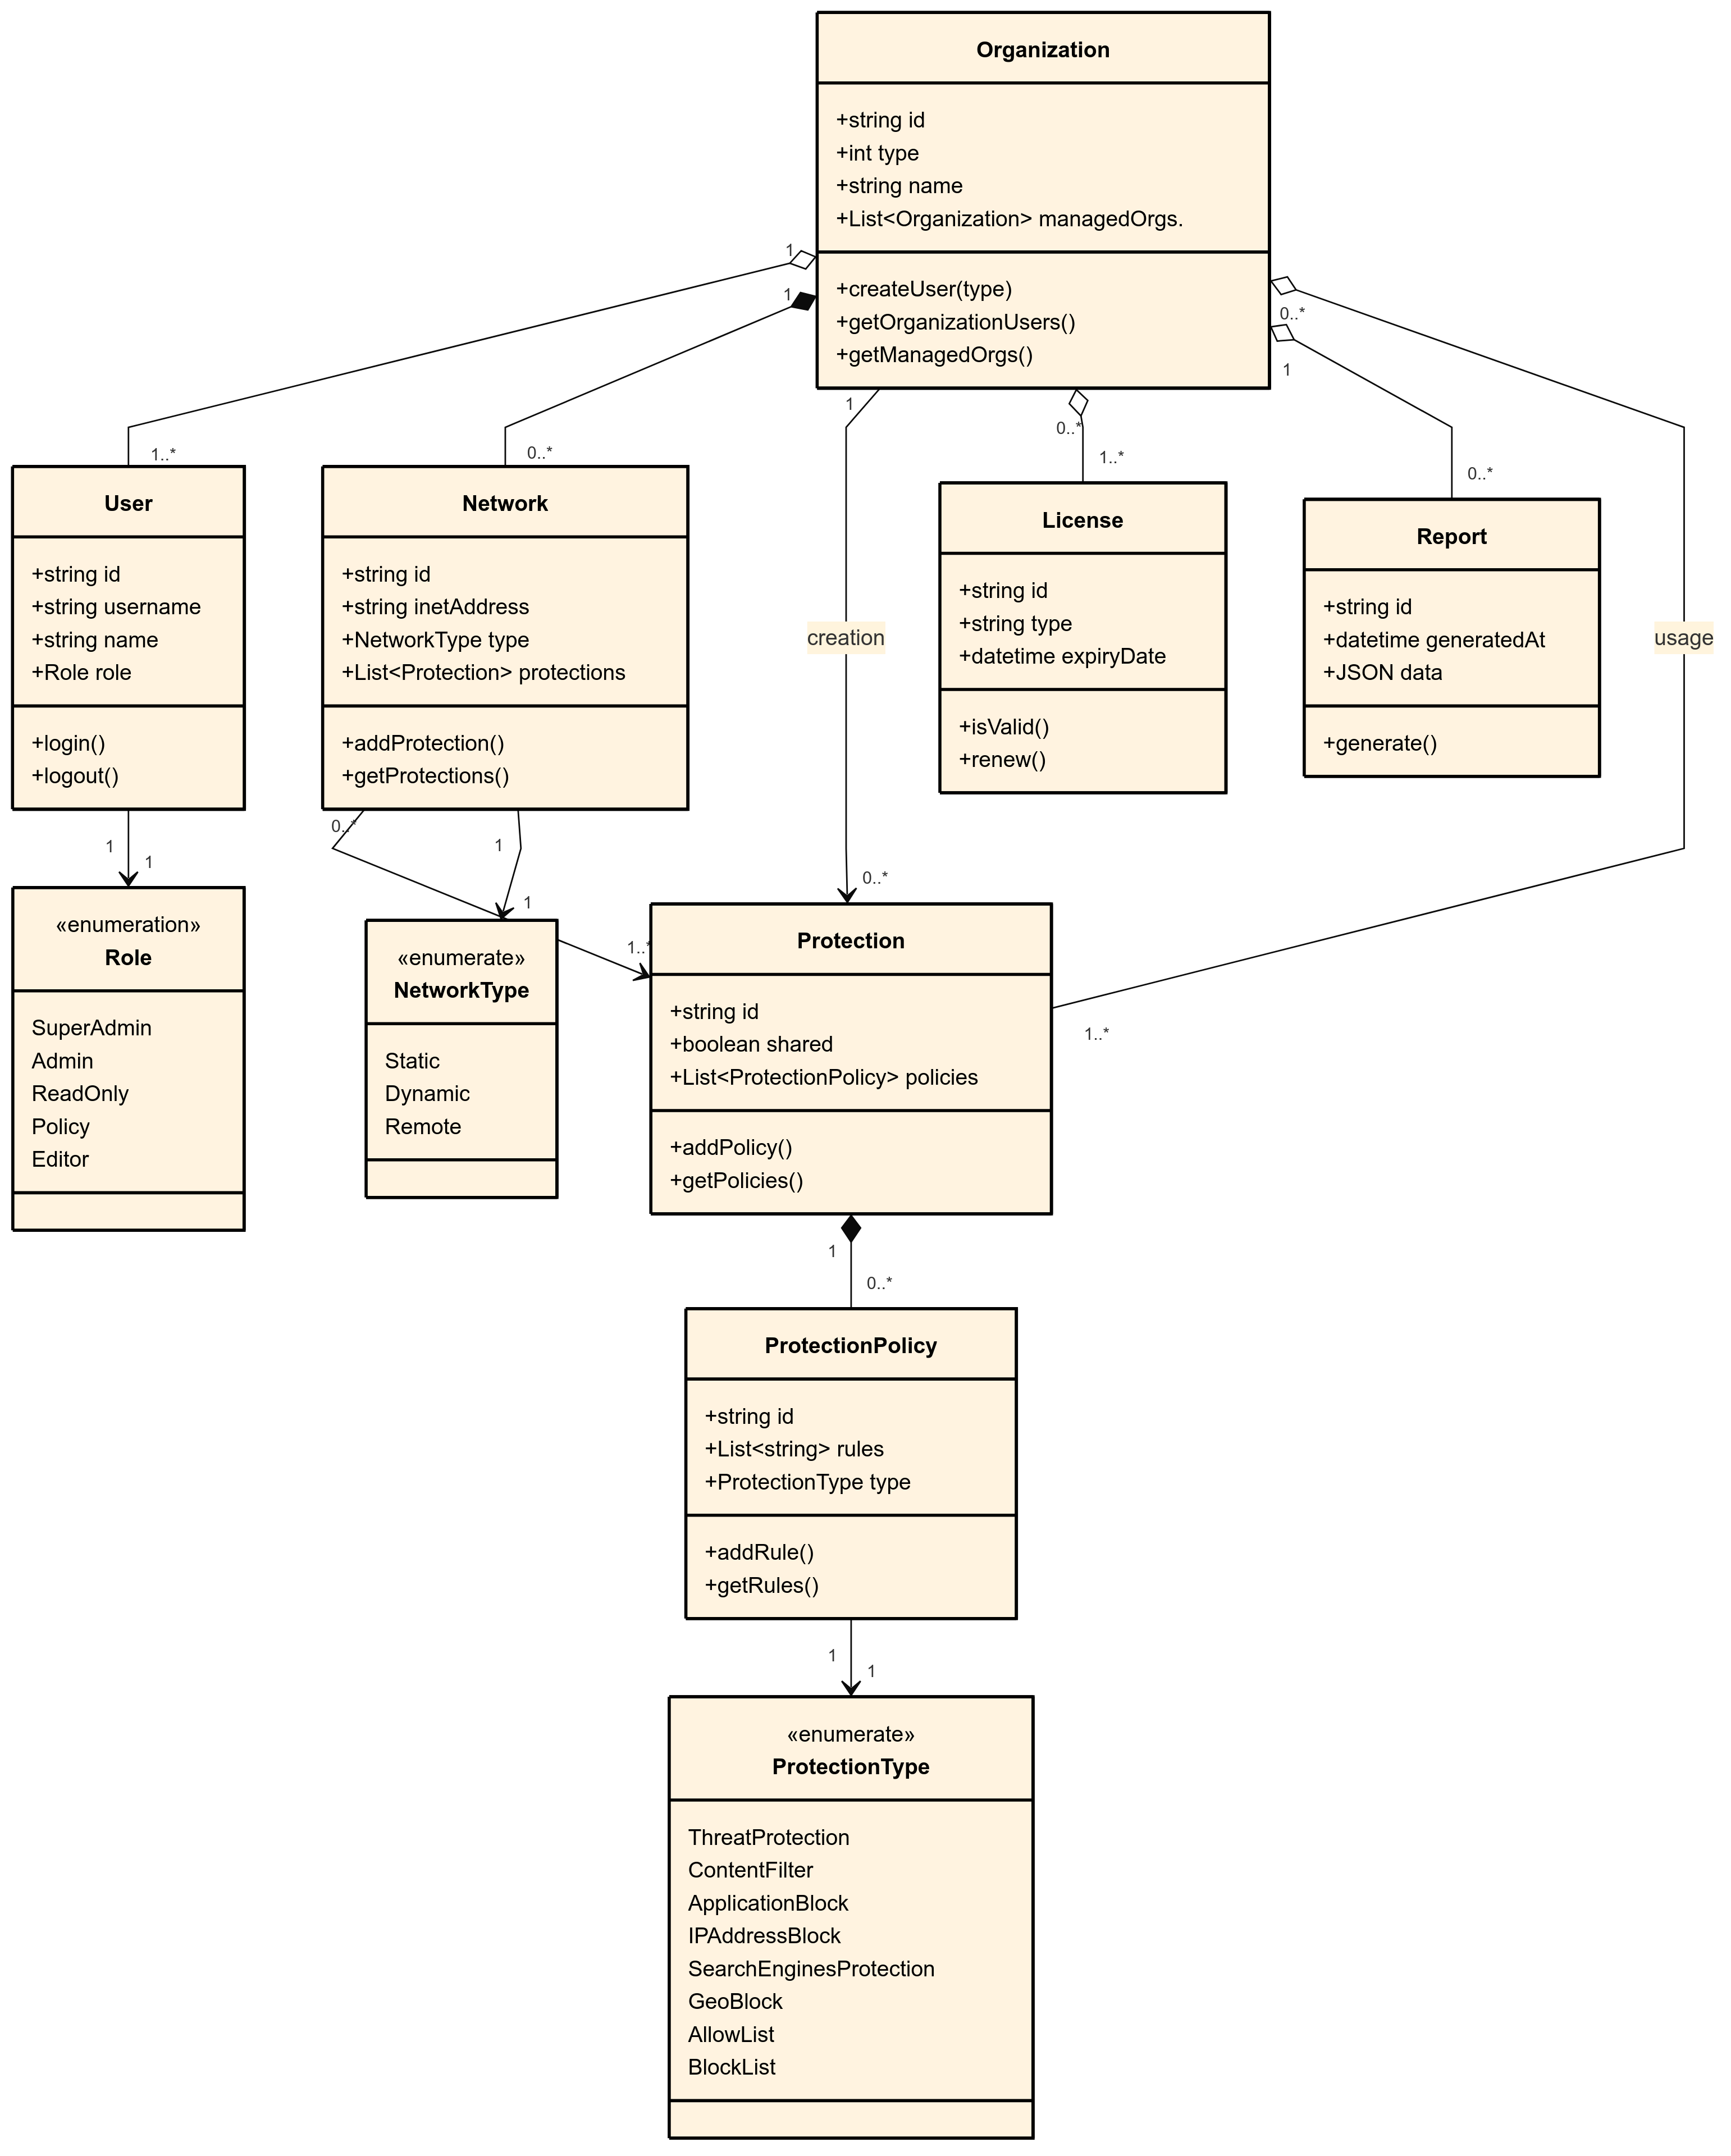
\includegraphics[width=1\textwidth]{figures/domain-model.png}
  \caption{Diagramma delle classi UML relativo al dominio applicativo del nuovo sistema.}
  \label{fig:domain_model}
\end{figure}

\subsubsection{Organization}
L'entità \texttt{Organization} rappresenta il fulcro del sistema multi-tenant ed è il punto di riferimento per tutte le altre componenti. Ogni utente, configurazione di filtraggio e reportistica è direttamente associato a un'organizzazione, che costituisce il contesto primario in cui avvengono le operazioni all'interno del sistema.

L'organizzazione è l'elemento che definisce l'esistenza stessa di un utente all'interno del sistema. Questi ultimi, infatti, non esistono al di fuori del contesto organizzativo: ogni utente deve appartenere a una specifica organizzazione e non può operare al di fuori di essa. Al momento della creazione di una nuova organizzazione, viene automaticamente generato un primo utente con permessi di amministratore. Tale amministratore ha la facoltà di creare nuovi utenti all'interno della propria organizzazione, o in quelle da essa gestite.

L'entità in questione non si limita a definire il perimetro degli utenti, ma è il nodo centrale attorno al quale ruotano tutte le altre configurazioni del sistema. Ogni organizzazione è associata a una o più reti (Network), che rappresentano gli indirizzi IP da sottoporre al filtraggio DNS. Le configurazioni di protezione (Protection), che definiscono cosa filtrare, sono legate all'organizzazione e non ai singoli utenti. Questo significa che tutte le policy di filtraggio sono decise a livello organizzativo. I dati statistici relativi all’utilizzo del sistema di filtraggio DNS sono raccolti e visualizzati a livello di organizzazione, consentendo agli utenti di monitorare il traffico filtrato e le attività correlate.

Ogni organizzazione è identificata da un \texttt{id} univoco, un nome (\texttt{name}) e una tipologia (\texttt{type}) che ne determina il ruolo all'interno del sistema. Esistono due macrotipologie di organizzazione:
\begin{itemize}
  \item \textbf{Organizzazioni che gestiscono altre organizzazioni}, ovvero Managed Service Provider e Dealer.
    \begin{itemize}
      \item \textbf{MSP}: oltre a rivendere il servizio di filtraggio DNS, si occupano direttamente della gestione della protezione per i loro clienti. In questo modello, il cliente finale non ha autonomia sulle proprie policy di protezione, in quanto è l'MSP a definirle e amministrarle.
      \item \textbf{Dealer}: rivendono il servizio di filtraggio DNS, ma senza occuparsi della configurazione delle policy. I clienti finali hanno piena libertà di gestione delle proprie protezioni.
    \end{itemize}
  \item \textbf{Clienti finali}, che possono essere:
    \begin{itemize}
      \item \textbf{Altre organizzazioni}, come scuole, hotel, aziende, attività commerciali.
      \item \textbf{Singoli individui}, che desiderano proteggere la propria rete domestica e i propri dispositivi personali.
    \end{itemize}
\end{itemize}

\subsubsection{User}
L'entità \texttt{User} rappresenta qualsiasi soggetto in grado di accedere al pannello di configurazione di un'organizzazione ed eseguire azioni sulla base dei permessi definiti dal proprio ruolo. Gli utenti operano sempre all'interno del contesto di un'organizzazione, non potendo esistere in modo indipendente. Il sistema adotta un modello a ruoli per differenziare le capacità operative di ciascun utente, limitandone o ampliandone i privilegi a seconda delle necessità organizzative.

Esistono cinque tipologie di utenti, ciascuna con permessi specifici nell'ambito della propria organizzazione:
\begin{itemize}
  \item \textbf{SuperAdmin}: rappresenta l'utente con i più alti privilegi possibili. Questo ruolo è riservato al team di supporto dell'azienda produttrice del filtro DNS e gode di accesso illimitato a tutte le organizzazioni registrate nel sistema. Un SuperAdmin può creare ed eliminare utenti e organizzazioni, modificare qualsiasi policy e visionare tutti i report disponibili, indipendentemente dal cliente a cui sono associati.
  \item \textbf{Admin}: è l'utente amministratore della propria organizzazione e di tutte quelle al di sotto di essa nella gerarchia. Ha pieno controllo sulle entità amministrate ed è l'unico utente con il permesso di creare nuovi account all'interno del proprio contesto organizzativo.
  \item \textbf{Policy}: ha la facoltà di gestire le reti (Network) e i profili di protezione (Protection) all'interno della propria organizzazione. Non dispone di permessi amministrativi e non può gestire gli utenti.
  \item \textbf{Editor}: ha privilegi simili all'utente di tipo Policy, ma con un ambito più ristretto. In particolare, può gestire solo le configurazioni di sicurezza, senza poter modificare le impostazioni delle reti.
  \item \textbf{ReadOnly}: è l'utente con il livello di accesso più limitato. Ha esclusivamente il permesso di visionare report e statistiche, senza poter modificare alcuna configurazione. Il suo ruolo è strettamente legato al monitoraggio passivo delle attività del filtro DNS per una data organizzazione.
\end{itemize}

Ogni utente è identificato da un \texttt{id}, un nome (\texttt{name}), un ruolo (\texttt{role}) e da uno \texttt{username}. Quest'ultimo campo contiene l'indirizzo email dell'utente ed è utilizzato per l'autenticazione all'interno del sistema.

\subsubsection{License}
L'entità \texttt{License} rappresenta una delle componenti ancora in fase di modellazione, ma il suo ruolo nel sistema è chiaro: essa determina il livello di servizio del prodotto associato a un'organizzazione e influisce sui permessi e sulle funzionalità disponibili per quest’ultima. Ogni organizzazione deve disporre di almeno una licenza attiva per poter usufruire del servizio di filtraggio DNS.

Esistono diverse tipologie di licenze, tra cui quelle di prova, che vengono fornite gratuitamente con lo scopo di illustrare e dimostrare le capacità del prodotto prima di un eventuale acquisto. Oltre alle licenze di prova, sono previste licenze a pagamento con diversi livelli di servizio, i cui dettagli non sono ancora stati completamente definiti.

L'assegnazione di una licenza può essere effettuata esclusivamente da un utente con il ruolo di SuperAdmin, oppure dall’Admin di un’organizzazione di tipo MSP o Dealer. Ciò significa che solo il produttore del software e gli intermediari autorizzati possono concedere o modificare una licenza per un'organizzazione cliente.

\subsubsection{Report}
L'entità \texttt{Report} rappresenta la capacità del sistema di generare e visualizzare dati analitici relativi all'attività di filtraggio DNS per una o più organizzazioni. Lo scopo principale di un report è quello di fornire un monitoraggio dettagliato sull'utilizzo del filtro, offrendo statistiche utili per comprendere il traffico di rete e l'efficacia delle policy di protezione adottate. Tra le informazioni contenute in un report vi sono, ad esempio, il numero di richieste DNS bloccate, le cinque categorie di siti più frequentemente filtrate, il numero di domini non risolti e altri indicatori rilevanti per la sicurezza della rete.

Una caratteristica distintiva del nuovo sistema è la possibilità di generare report aggregati, che includono dati provenienti da più organizzazioni. Questa funzionalità è particolarmente utile per gli MSP, in quanto consente loro di ottenere una panoramica completa e centralizzata sui clienti che gestiscono. I report aggregati possono includere informazioni come l’elenco dei malware rilevati e i dispositivi su cui sono stati identificati, il numero di sessioni attive e altre metriche relative alla sicurezza e alla gestione del traffico DNS.

L'entità Report non è ancora stata completamente modellata, ma il suo ruolo nel sistema è fondamentale per garantire una visibilità chiara e approfondita sull’efficacia delle configurazioni di filtraggio applicate alle reti delle organizzazioni.

\subsubsection{Protection}
L'entità \texttt{Protection} rappresenta il concetto di protezione associato a una rete (Network), determinando in che modo il sistema di filtraggio DNS deve bloccare o consentire l'accesso ai contenuti. Ogni istanza di Protection è composta da una lista di policy di sicurezza, ognuna delle quali specifica una particolare configurazione del filtro. Generalmente, una Protection viene creata da un'organizzazione e assegnata a una o più delle proprie reti, definendo le regole di filtraggio applicate al traffico generato da tali indirizzi IP.

Con lo sviluppo del nuovo sistema, l’entità in esame introduce un'importante evoluzione: la possibilità di essere condivisa tra più organizzazioni. Se un’Organization crea una Protection e la contrassegna come condivisibile, tale configurazione potrà essere visualizzata e assegnata dai clienti gestiti dall'organizzazione creatrice. Questa funzionalità risulta particolarmente utile per gli MSP e i Dealer, che possono fornire ai propri clienti configurazioni predefinite e standardizzate senza richiedere loro di crearne di nuove.

Un ulteriore vantaggio del nuovo modello è la propagazione automatica delle modifiche per le Protection condivise. Se l’organizzazione creatrice aggiorna una configurazione di protezione condivisa, tutte le organizzazioni che la utilizzano vedranno applicate automaticamente le modifiche senza necessità di intervento manuale. Per supportare questa logica, la modellazione prevede due relazioni distinte tra Protection e Organization:
\begin{enumerate}
  \item Una relazione di \textit{associazione semplice} che esprime la creazione, collegando un’Organization alla Protection che ha generato.
  \item Una relazione di \textit{aggregazione} che esprime l’utilizzo, collegando una Protection a una o più Organization che la utilizzano. Questa relazione è valida sia per le Protection non condivise, che per quelle condivise.
\end{enumerate}

Nonostante la sua importanza, Protection da sola non è sufficiente a garantire il livello di granularità richiesto da un moderno sistema di filtraggio DNS. Per questo motivo, essa è composta da una lista di configurazioni più specifiche, rappresentate dall'entità ProtectionPolicy, che definisce nel dettaglio il comportamento della protezione.

\subsubsection{ProtectionPolicy}
L'entità \texttt{ProtectionPolicy} rappresenta un insieme di regole appartenenti alla stessa tipologia di protezione, definita dall'attributo \texttt{ProtectionType}. Poiché il sistema di filtraggio DNS prevede diverse categorie di protezione, la modellazione adotta una struttura a due livelli: l'entità Protection mantiene la lista delle policy applicate, mentre ogni elemento di questa lista (ProtectionPolicy) contiene le regole specifiche relative a una determinata categoria di protezione.

Questa suddivisione consente di organizzare in modo chiaro e modulare le configurazioni di sicurezza. Un'istanza di Protection può essere composta da più ProtectionPolicy, ciascuna responsabile di un particolare aspetto del filtraggio. Questo approccio permette alle organizzazioni di combinare diverse policy all'interno di un'unica configurazione di protezione, garantendo così una gestione flessibile e scalabile delle regole di filtraggio DNS.

I possibili tipi di protezione (ProtectionType) includono:
\begin{itemize}
  \item \textbf{ThreatProtection}: blocca siti identificati come minacce alla sicurezza, come malware e phishing.
  \item \textbf{ContentFilter}: filtra i contenuti sulla base della loro categoria tematica (es. pornografia, giochi d'azzardo, social network).
  \item \textbf{ApplicationBlock}: impedisce l’accesso a specifiche applicazioni o servizi online.
  \item \textbf{IPAddressBlock}: blocca l'accesso a determinati indirizzi IP.
  \item \textbf{SearchEnginesProtection}: applica restrizioni alle ricerche sui motori di ricerca, come l'attivazione forzata della modalità SafeSearch.
  \item \textbf{GeoBlock}: limita l’accesso a domini o indirizzi IP in base alla loro geolocalizzazione.
  \item \textbf{AllowList} e \textbf{BlockList}: definiscono eccezioni personalizzate, rispettivamente per consentire o bloccare domini specifici.
\end{itemize}

\subsubsection{Network}
L'entità \texttt{Network} riveste un ruolo fondamentale nel presente dominio applicativo, in quanto definisce l’ambito su cui devono essere applicate le regole di protezione del filtro DNS. Ogni rete è associata a un'Organization e rappresenta il punto di ingresso del traffico che verrà sottoposto a filtraggio. La configurazione della protezione di una rete è determinata dalla Protection assegnata ad essa, specificando così quali policy devono essere applicate.

Questa relazione tra Network e Organization è modellata come una \textit{composizione}, indicando che una rete non può esistere senza l’Organization a cui appartiene. Se un'organizzazione viene eliminata, anche tutte le reti ad essa associate vengono rimosse.

Una rete può appartenere a una delle seguenti tipologie, identificate dall'enumerazione \texttt{NetworkType}:
\begin{itemize}
  \item \textbf{Static}: identifica reti con un indirizzo IP statico, il cui riferimento rimane invariato nel tempo.
  \item \textbf{Dynamic}: rappresenta reti con indirizzo IP dinamico, che necessitano dell’ausilio di un servizio di DynamicDNS per garantire un'associazione stabile nel tempo.
  \item \textbf{Remote}: utilizzata per proteggere dispositivi mobili ed endpoint aziendali che richiedono la protezione del filtro DNS anche quando non sono connessi alla rete principale dell'organizzazione.
\end{itemize}

Ogni Network è identificata da un \texttt{id}, da un \texttt{type} e da un \texttt{inetAddress}. Quest'ultimo supporta sia indirizzi IPv4 che IPv6 e consente l'inserimento di intervalli IP secondo lo standard CIDR\footnote{\url{https://datatracker.ietf.org/doc/html/rfc4632}}, specificandoli con una barra finale (es. \texttt{192.168.1.0/24}). L'associazione tra \texttt{Network} e \texttt{Protection} permette di applicare un insieme di policy a una specifica rete, garantendo così un controllo granulare sul filtraggio del traffico DNS.
